\bartchapterimage{heic0911c.jpg}
\chapter{Density profiles}
\label{cha:profiles}
\bartthumb{heic0911c.png}

\section{Introduction}

In this chapter, there is some details on the computation of the density
profiles and there derived quantities. We define here the different
normalization used along the thesis for some useful current density profiles.

\subsection{Definitions}

The number of galaxies in a sphere of radius $r$ with a density profile in
number $\nu(r)$ is the case of a spherical symmetry:
%
\begin{equation}
    N\left(r\right)=\int_0^r4\pi {r'}^2 \nu(r')\dd{r'}
\end{equation}

To start, we define some functions with no dimension used to make easier some
computations.
%
\begin{eqnarray}
    N\left(r\right)&=N\left(a\right){\widetilde{N}\left(r/a\right)}\nonumber\\
    \nu\left(r\right)&=
        \frac{N\left(a\right)}{4\pi{a^3}}
        \widetilde\nu\left(r/a\right)\nonumber\\
\end{eqnarray}
%
with $a$ the radius at which the slope of the density profile is equal to -2 in
logarithmic space. We also define the same relations for a virial
normalization.
%
\begin{eqnarray}
    N\left(r\right)&={N_v}{\overline{N}\left(r/\rvir\right)}\nonumber\\
    \nu\left(r\right)&=
        \frac{N_v}{4\pi\rvir^3}\overline\nu\left(r/\rvir\right)\nonumber\\
\end{eqnarray}

We also define the concentration $c$ as the ratio between the virial radius
$\rvir$ and the radius $a$, i.e.\ $c=\rvir/a$.

\section{Density profiles}
\label{sec:density_profiles}

\subsection{\citet{NFW+97}}

The definition of a NFW profile is:
%
\begin{equation}
    \nu \left(r\right) = \cfrac{\nu_0}{r {\left(r+a\right)}^2}
\end{equation}
%
with $\nu_0$ a constant.

We can write by integrating previous relations and searching for the constant
$\rho_0$:
%
\begin{equation}
    \widetilde\nu\left(x\right)=\cfrac{1}{\ln2-1/2}
        \quad\cfrac{1}{x{\left(1+x\right)}^2}
\end{equation}
%
\begin{equation}
    \widetilde{N}\left(x\right)=\cfrac{1}{\ln2-1/2}
        \quad\left(\ln\left(1+x\right)-\cfrac{x}{x+1}\right)
\end{equation}
%
\begin{equation}
    \overline\nu\left(x\right)=
        \cfrac{1}{\ln\left(1+c\right)-c/ \left(1+c\right)}
        \quad\cfrac{1}{x{\left(1/c+x\right)}^2}
\end{equation}
%
\begin{equation}
    \overline{N}\left(x\right)=
        \cfrac{1}{\ln \left(1+c\right)-c/ \left(1+c\right)}
        \quad\left(\ln\left(1+xc\right)-\cfrac{xc}{xc+1}\right)
\end{equation}

\subsection{Einasto}
\label{sub:einasto}

For an Einasto density profile:
\begin{equation}
    \nu \left(r\right) = \nu_0 \exp
    \left(- {\left(\cfrac{r}{b}\right)}^{1/m}\right)
\end{equation}

Writing the definition of the $a$ radius with this density profile, we have:
%
\begin{equation}
    {\left(\cfrac{1}{b}\right)}^{1/m} = 2m{\left(\cfrac{1}{a}\right)}^{1/m}
\end{equation}
%
leading to the following normalizations:
%
\begin{equation}
    \widetilde\nu \left(x\right) = \cfrac{{\left(2m\right)}^{3m}}{m\gamma
    \left(3m, 2m\right)} \exp \left(-2mx^{1/m}\right)
\end{equation}
%
\begin{equation}
    \widetilde{N} \left(x\right) = \cfrac{\gamma \left(3m, 2m
    x^{1/m}\right)}{\gamma \left(3m, 2m\right)}
\end{equation}
%
\begin{equation}
    \overline\nu \left(x\right) = \cfrac{{\left(2m\right)}^{3m}}{m\gamma
    \left(3m, 2m c^{1/m}\right)} \exp \left(-2m{\left(xc\right)}^{1/m}\right)
\end{equation}
%
\begin{equation}
    \overline{N} \left(x\right) = \cfrac{\gamma \left(3m, 2m
        {\left(xc\right)}^{1/m}\right)}{\gamma \left(3m, 2m c^{1/m}\right)}
\end{equation}

\subsection{Generalized NFW}
\label{sub:generalized_nfw}

If any previous density profiles isn't sufficient to describe the distribution
of dark matter particles or galaxies inside the halos, a solution is possibly
to fit a generalized NFW profile, whose the density is:
%
\begin{equation}
    \nu \left(r\right) =
    \cfrac{\nu_0}{r^\alpha{\left(r+a\right)}^{\beta-\alpha}}
\end{equation}

In this case:
%
\begin{equation}
    \widetilde{N} \left(x\right) = \cfrac{%
        \mathcal{B}_{-x} \left(3-\alpha, 1+\alpha-\beta\right)}
    {\mathcal{B}_{-1} \left(3-\alpha, 1+\alpha-\beta\right)}
\end{equation}
%
\begin{equation}
    \widetilde\nu \left(x\right) = \cfrac{1}
    {{\left(-1\right)}^{\alpha+1}
        \mathcal{B}_{-1} \left(3-\alpha, 1+\alpha-\beta\right)}
    \quad\cfrac{1}
    {x^\alpha {\left(1+x\right)}^{\beta-\alpha}}
\end{equation}
%
and for the virial normalization:
%
\begin{equation}
    \overline{N} \left(x\right) = \cfrac{%
        \mathcal{B}_{-xc} \left(3-\alpha, 1+\alpha-\beta\right)}
    {\mathcal{B}_{-c} \left(3-\alpha, 1+\alpha-\beta\right)}
\end{equation}
%
\begin{equation}
    \overline\nu \left(x\right) = \cfrac{1}
    {{\left(-1\right)}^{\alpha+1}
        \mathcal{B}_{-c} \left(3-\alpha, 1+\alpha-\beta\right)}
    \quad\cfrac{1}
    {{\left(xc\right)}^\alpha {\left(1+xc\right)}^{\beta-\alpha}}
\end{equation}
%
where $\mathcal{B}$ is the function defined as:
%
\begin{equation}
    \mathcal{B} \left(a, b\right) =
    \cfrac{\Gamma \left(a\right) \Gamma \left(b\right)}
    {\Gamma \left(a+b\right)} =
    \int_0^1 t^{a-1} {\left(1+t\right)}^{b-1} \dd t
\end{equation}
%
and its incomplete version is:
%
\begin{equation}
    \mathcal{B}_z \left(a, b\right) =
    \int_0^z t^{a-1} {\left(1+t\right)}^{b-1} \dd t
\end{equation}

\section{Radial velocity dispersion}
\label{sec:radial_velocity_dispersion}

Galaxies in groups (and their associated dark matter halos) are assumed to be a
system of particles only submitted to the gravitation. Neglecting mergers and
other physical processes inside galaxy groups, the number of galaxies doesn't
evolve in phase space, and the distribution function is constant along the
evolution of the system. In this case, we can use the Boltzmann equation
without collisions to extract dynamical properties of galaxy groups.

The Jeans equation is a particular case of the Boltzmann equation, assuming a
spherical symmetry of the system and stationarity. It is expressed as:
%
\begin{equation}
    \label{eq:jeans}
    \ddp{\left(\nu(r)\sigma_r^2(r)\right)}{r} + \cfrac{2\mybeta}{r}\left(\nu(r)\sigma_r^2(r)\right)=
    -\nu(r)\cfrac{GM(r)}{r^2}
\end{equation}

We can compute the radial velocity dispersion using \bartrefequation{jeans} for
a spherical system at equilibrium. The solution to this equation is given by:
%
\begin{equation}
    \myprofil\sigma_r^2(r)=\int_r^\infty K_r(r,s)\nu(s)\cfrac{GM(s)}{s^2}\dd{s}
\end{equation}
%
with $K_r(r,s)$ the kernel of the integral defined as:
%
\begin{equation}
    K_r(r,s)=\exp\left[2\int_r^s\mybeta\cfrac{\dd{t}}{t}\right]
\end{equation}

There is two ways of normalizing the radial velocity dispersion according to
the normalization used for the density and mass profiles. We show it for the
virial normalization for illustration:
%
\begin{equation}
    \label{eq:sigma_norm}
    \overline\sigma_r^2(x)= \cfrac{1}{\overline\nu \left(x\right)}
    \int_x^\infty K_r(x,s)\overline\nu(s)\cfrac{\overline{M}(s)}{s^2}\dd s
\end{equation}
%
with:
%
\begin{equation}
    \sigma_r^2(r) = \cfrac{GM_v}{\rvir}\overline\sigma_r^2(r/\rvir)
\end{equation}

We are interested only in the NFW profile in the thesis, since it is accurate
enough to adjust the model. If we want analytical form, we need to choose the
model we want for the anisotropy profile. We provide here some expressions of
the radial velocity dispersion, assuming the NFW density profile, for some
anisotropy models.

\subsection{\citet{ML+05}}
\label{sub:ml05}

This model is of the form:
%
\begin{equation}
    \beta \left(r\right) = \undemi\cfrac{r}{r+b}
\end{equation}
%
where $b$ is a characteristic radius of the model. Introducing this expression
in \bartrefequation{sigma_norm}, we obtain:
%
\begin{align}
    \widetilde\sigma_r^2(x)=&
        -\frac{1}{3 x (1+r x)
        {(-1+\ln\left(4\right))}^2}2
        \left(-\frac{1}{2}+\ln\left(2\right)\right)\nonumber\\
    &\left(x \left(3+x \left(\pi ^2 (-3+2 r)
        {(1+x)}^2-3 (-9+5 r-7 x+4 r x)
        \right)\right.\vphantom{\ln\left(1+\frac{1}{x}\right)}\right.
        \nonumber\\
    &\left.-3 x^3 \ln\left(1+\frac{1}{x}\right)+3 x (1+2 x)
        \ln\left(x\right)\right)\nonumber\\
    & -3 (1+2 x (-1-2 x (2+x)+r (1+x) (1+2 x)))
        \ln\left(1+x\right)+3 (-3+2 r) {\left(x+x^2\right)}^2
        \ln{\left(1+x\right)}^2\nonumber\\
    & \left.+6 (-3+2 r) x^2 {(1+x)}^2
        Li_2\left(-x\right)\vphantom{\ln\left(1+\frac{1}{x}\right)}\right)
        \nonumber\\
\end{align}
\begin{align}
    \widetilde\sigma_r^2(x)=&
        \frac{1}{6 x (1+r x) \left(-1+\frac{1}{1+c}+\ln\left(c\right)\right)}
        \left(c x \left(-3+x \left(3 c \left(-9+\pi ^2\right)+
        \left(15-2 \pi ^2\right) r\right.\right.
        \vphantom{{(1+c x)}^2}\right.\\
    &\left. -4 c \left(-3+\pi ^2\right) r x+
        3 c^3 \pi ^2 x^2+c^2 x \left(-21+\pi ^2 (6-2 r x)\right)\right)\\
    & \left.+6 c^3 x^3 {\rm arccoth} \left(1+2 c x\right)-
        3 c x (1+2 c x) \ln\left(c x\right)\right)\\
    &+3(1+2 x (r+c (-1+x (-4 c+3 r+2 c (-c+r) x))))
        \ln\left(1+c x\right)\\
    &\left.+3c(3 c-2 r) x^2 {(1+c x)}^2 {\left(\ln\left(1+c x\right)\right)}^2+
        6 c (3 c-2 r) x^2 {(1+c x)}^2 Li_2\left(-c x\right)\right)\\
\end{align}

\section{Line of sight velocity variance}

We will compute in this section the line of sight velocity dispersion of
galaxies in a general spherical density profile, and then compute it
specifically for an NFW profile. This useful to make cuts at some sigma in the
velocity profile to check where is the most important part of a group.

By definition, the variance is the mean of the squared quantity under the
assumption of a distribution function. We use a general density profile which
is invariant under rotations $\nu{(r)}$. In our case, we make this mean on the
line of sight, so:
%
\begin{equation}
    \sigma_{LOS}^2\left({R}\right)=\cfrac{\int_{-\infty}^{\infty}{v_{LOS}^2}\nu{(r)}\dd{z}}
    {\int_{-\infty}^{\infty}\nu{(r)}\dd{z}}
\end{equation}
%
But in the group $r^2=R^2+z^2$ so:
%
\begin{equation}
    \sigma_{LOS}^2\left({R}\right)=\cfrac{2\int_{R}^{r_{\max}}{v_{LOS}^2}\cfrac{\nu{(r)}{r}}{\sqrt{r^2-R^2}}\dd{r}}
    {2\int_{R}^{r_{\max}}\cfrac{\nu{(r)}{r}}{\sqrt{r^2-R^2}}\dd{r}}
\end{equation}
%
The denominator is by definition the projected density surface along the line
of sight and we denote it
%
\begin{equation}
    \Sigma(R) = 2\int_{R}^{r_{\max}}\cfrac{\nu{(r)}{r}}{\sqrt{r^2-R^2}}\dd{r}
\end{equation}
%
Normally the integration is for $r_{\max}\rightarrow\infty$ but in our case we
want to restrict to a limited region in the group (to virial sphere precisely).

In the same coordinate system as previously, the line of sight velocity can be
expressed in spherical coordinates as:
%
\begin{equation}
    v_{\mathrm{LOS}} = v_r \cos\theta - v_\theta \sin\theta
\end{equation}
%
We suppose that we are at the equilibrium and so that there is no flow in the
group in consequence we can neglect means of velocities. In terms of velocity
variance we have now:
%
\begin{equation}
    \mysigma\mysiglos = 2\int_R^{r_{\max}}
    \left({\sigma_r^2(r)\cos^2\theta+\sigma_\theta^2\sin^2\theta}\right)
    \cfrac{\nu{(r)}{r}}{\sqrt{r^2-R^2}}\dd{r}
\end{equation}
%
If we want to use the anisotropy parameter
$\mybeta=1-\sigma_\theta^2(r)/\sigma_r^2(r)$ in case of sphericity, we can
write:
%
\begin{equation}
    \mysigma\mysiglos = 2\int_R^{r_{\max}}
    \left({1-\mybeta\cfrac{R^2}{r^2}}\right)
    \cfrac{\nu{(r)}{\sigma_r^2(r)}{r}}{\sqrt{r^2-R^2}}\dd{r}
\end{equation}

We can compute the radial velocity dispersion using the Jeans equation for a
spherical system at equilibrium.
%
\begin{figure}[H]
    \centering
    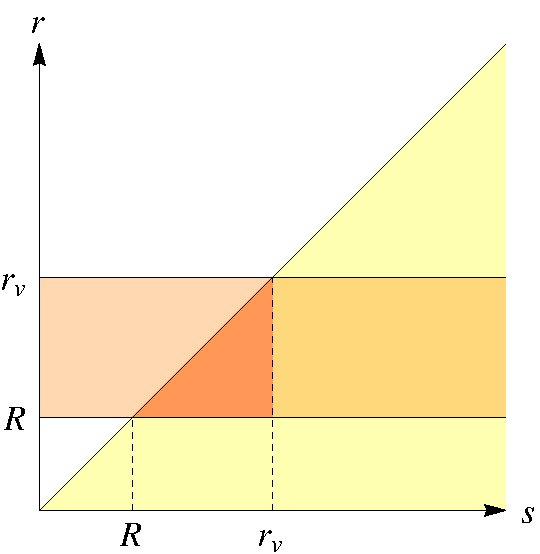
\includegraphics[width=0.5\linewidth]{figures/los_variance/domint}
    \caption{Integration domain for the line of sight radial
    dispersion.\label{fig:domint}}
\end{figure}

\subsection{Supposing \citet{Mamon+05} anisotropy}

With the decomposition of the integral over the domain of integration (see
\bartreffigure{domint}), we can write:
%
\begin{eqnarray}
    &&\Sigma{(R)}{\sigma_{LOS}}^2{(R)}=
        2\int_R^{r_v}{\frac{\left({s+a}\right)}{s^2}{\nu(s)}{G}{M(s)}}{\dd{s}}
        \nonumber\\
    &\times&
        \left(\int_R^s{\left(\frac{r}{r+a}-\undemi
        {\left(\frac{R}{r+a}\right)}^2\right)
        \frac{1}{\sqrt{r^2-R^2}}\dd{r}}\right)\nonumber\\
    &+&2\int_{r_v}^{\infty}
        \frac{\left({s+a}\right)}{s^2}\nu(s){G}{M(s)}\dd{s}\nonumber\\
    &\times&
        \left(\int_R^{r_v}
            \left(\frac{r}{r+a}-\undemi{\left(\frac{R}{r+a}\right)}^2\right)
            \frac{1}{\sqrt{r^2-R^2}}\dd{r}\right)\nonumber\\
\end{eqnarray}
%
where we are setting $r_{\max}$ to $r_v$. So now we can write using the
fact that $4a\nu(a)\widetilde{\Sigma}(R/a,c)$:
%
\begin{eqnarray}
    &&{\sigma_{LOS}}^2{(R)}={v_v}^2\frac{c/2}{\widetilde{M}{(c)}\widetilde{\Sigma}{(R/a,c)}}\nonumber\\
    &\times&\left(\int_{R/a}^c{{K}\left({x\frac{a}{R},\frac{a}{R}}\right)}\widetilde{\nu}{(x)}
    \frac{\widetilde{M}{(x)}}{x}\dd{x}+I\left({c\frac{a}{R},\frac{a}{R}}\right){J(c)}\right)\nonumber\\
\end{eqnarray}
%
\begin{equation}
    I(u,u_a)=\left\{\begin{array}{lr}
        -u_a{\rm{sign}}(u_a-1)\frac{{u_a}^2-1/2}{|{u_a}^2-1|^{3/2}}{C^{-1}\left(\frac{1+u{u_a}}{u+u_a}\right)}&\\
        \hspace{5em}+{\rm{acosh}}{u}+\frac{1/2}{u_a+u}\frac{\sqrt{u^2-1}}{{u_a}^2-1},&{u_a}\neq1\\
        {\rm{acosh}}{u}-\sqrt{\frac{u-1}{u+1}}\left(\frac{8+7u}{6(1+u)}\right),&{u_a}=1\\
    \end{array}\right.
\end{equation}
%
with:
%
\begin{equation}
    K(u,u_a)=\left({1+\frac{u_a}{u}}\right){I(u,u_a)}
\end{equation}
%
and:
%
\begin{equation}
    C^{-1}(X)=\left\{\begin{array}{lr}
        {\rm{acosh}}{X}&u_a>1\\
        {\rm{acos}}{X}&u_a<1\\
    \end{array}\right.
\end{equation}
%
We have too an other integral:
%
\begin{equation}
    J(y)=\int_y^{\infty}\frac{x+1}{x^2}\widetilde{\nu}{(x)}\widetilde{M}{(x)}\dd{x}
\end{equation}
%
In the case of an NFW profile, this can be expressed in an analytical way:
%
\begin{align*}
    J(y)&=
        \frac{2}{3{y^2}(1+y){\left(\ln{4}-1\right)}^2}
        \left(y\left(-3+y\left(-9+\pi^2\left(1+y\right)\right)\right)\right.\\
    &+3{y^3}\ln\left(1+\frac{1}{y}\right)+3\ln\left(1+y\right)
            \left(1-y+y^2\left(1+y\right)\ln\left(1+y\right)\right)\\
    &\left.-3{y^2}\ln\left({y}\left(1+y\right)\right)+6{y^2}
        \left(1+y\right){\dilog{-y}}\right)\\
\end{align*}
%
where the dilogarithm function is defined in our case as:
%
\begin{equation}
    \dilog{z}=-\int_0^1\cfrac{\ln{(1-zt)}}{z}\dd{t}
\end{equation}

Still in the case of the NFW profil, in \citet{MBM+10} there is the expression
of $\widetilde{\Sigma}$:
%
\begin{multline}
    \widetilde{\Sigma}(X,c)=\cfrac{1}{2\ln2-1}\int_X^c\cfrac{\dd{x}}{{(1+x)}^2\sqrt{x^2-X^2}}\\
    =\cfrac{1}{2\ln2-1}\begin{cases}
        \cfrac{1}{{(1-X^2)}^{3/2}}
        \cosh^{-1}\left[\cfrac{c+X^2}{(c+1)X}\right]-
        \cfrac{1}{(c+1)}\cfrac{\sqrt{c^2-X^2}}{1-X^2} &\text{if } 0<X<1 \\
    \cfrac{\sqrt{c^2-1}(c+2)}{3{(c+1)}^2} &\text{if } X=1<c\\
    \cfrac{1}{(c+1)}\cfrac{\sqrt{c^2-X^2}}{X^2-1}-
    \cfrac{1}{{(X^2-1)}^{3/2}}
    \cos^{-1}\left[\cfrac{c+X^2}{(c+1)X}\right] &\text{if } 1<X<c\\
    0 &\text{if } X=0\text{or}X>c
    \end{cases}
\end{multline}

% vim: set tw=79 : set concealcursor=
